

\label{sub:SpecO}


Our assertion language %\AssertLang, 
{supports} standard  as well \emph{object-capability} assertions. 
 The  standard assertions  include the values of fields, implication, quantification etc, as well as ghost fields; the latter can represent user-defined predicates. 
The  object capability assertions express restrictions of an object's eventual authority on some other object.
{They are about objects being
\emph{external} or about   \emph{protection} -- inspired by the OCAP literature.}
\footnoteSD{TODO say how these relate with capability lit;  compare with 
 OOPSLA.}
%We define the meaning of  standard'' assertions in section \ref{sect:semantics:assert:standard}, 
%and the meaning of the   object-capability assertions in  sections \ref{sect:semantics:assert:prtFrom}
%and  \ref{sect:semantics:assert:prt}.


%\subsection{Syntax of \AssertLang}
%The syntax of \AssertLang  is given in Definition \ref{f:chainmail-syntax}.
%Standard assertions may be  extended expressions,   queries on an object's class, or the usual connectives and quantifiers. 
%{Extended expressions, $\re$, may include addresses -- the reason is discussed later.}

%\susan{why extended expression rather than just expression?}

\begin{definition}
\label{def:assert:syntax}
Expressions, $\re$, and assertions, $A$,  are defined as follows:

\label{f:chainmail-syntax}
 \[
\begin{syntax}
\syntaxElement{\re}{}
		{
		\syntaxline
				{\prg{true}}
				{{\alpha}}
				{{x}}
				{\re.f}
				{\re.f({\overline{\re}})}
		\endsyntaxline
		}
\endSyntaxElement
\\
\syntaxElement{A}{}
		{
		\syntaxline
				{{\re}}
				{{\re} : C}
				{\neg A}
				{A\ \wedge\ A}
		%		{A\ \vee\ A}
				{\all{x:C}{A}}
		%		{\ex{x:C}{A}}
%		\endsyntaxline
%		}
% 		{
% 		\syntaxline
				{\external{{\re}}}
 %				{\external{{\re}}}
				{\protectedFrom{{\re}} {{\re}}} 
				 {\inside {{\re}}} 
		\endsyntaxline
		}
\endSyntaxElement\\
\end{syntax}
\]
In the above, we expect that $f$ stands  for a field or a ghost field, but not a method -- \ie no side-effects. {{Moreover, $\fv(A)$ is defined in the obvious way to to return   the free variables in $A$; for example, $\fv(a\!:\!Account \wedge \forall b:int.[a.\balance = b])$=$\{ a \}$.}}
\end{definition}

\noindent
\textbf{NOTES}  \notesep % Extended expressions, $\re$, and therefore also 
 Assertions  may contain addresses; \eg   $\alpha.bal > 700$. 
{While addresses make little sense in user-written assertions, they are useful when giving semantics to universal quantifiers 
\cf Def. \ref{def:chainmail-semantics}.(\ref{quant1}), {when the local map changes \eg upon call and return, and in general,} for two-state invariants, \cf Def. \ref{def:necessity-semantics}.(2).}
\notesep The syntax does  not distinguish between fields and ghost fields. For instance, $\prg{a}.\prg{\balance}$ may, in some modules (\eg in \ModA), be a field lookup, while in others (e.g. when the balance is defined though an entry in a lookup table) may involve executing a ghost function. 
% -  $\external {\re}$ is short for $\neg \internal {\re}$. We use these forms freely in the subsequent text without further definition.
%\kjx{These NOTES seem to make heavy work of mostly trivial points
%{{SD: WIll work on that}}
% \footnoteSD{{\textbf{NOTE for us} It also allows assertions like $a1.passwd \neq a2.passwd$, whereas in the past we would have written as $\exists x,y.[\ a1.passwd=x \wedge  a2.passwd=y \wedge x\neq y\ ]$.}} \footnoteSD{{TODO compare with oopsla }}


\begin{definition}[Shorthands] 
\sdN{We use $\internal {\re}$ as short for $\neg (\internal {\re})$}, and
$\extThis$. resp. \sdN{$\intThis$} as  short  for $\external{\prg{this}}$, resp. $\internal{\prg{this}}$.%, and $\re:\prg{intl}$ as short for $ \neg \external {\re}}$. 
The forms $A \rightarrow A'$, or $A \vee A'$, or $\exists x:C.A$  can be encoded; we use these forms freely in the subsequent text.
% without further definition.
\end{definition}



\begin{definition}[Satisfaction  of Assertions by module and  state] 
\label{def:chainmail-semantics-all}
\label{def:chainmail-semantics}
is expressed through  through \ \ $\satisfiesA{M}{\sigma}{{A}}$ \ \ \ and defined by cases on the shape of $A$, in definitions \ref{def:chainmail-semantics}, \ref{def:chainmail-protection-from}, and 
 \ref{def:chainmail-protection}.
\end{definition}

\footnoteSD{say why we split the def into three defs.} 
\noindent
\textbf{NOTE}  While execution takes place in the context of one or more modules, $\Mtwo$, satisfaction of assertions considers \emph{exactly one} module  $M$ -- the internal module. 
%{This is not surprising since the goal of this work is to ensure that external modules cannot break our (internal) module's assertions.}
%\footnoteSD{We need to have clarified internal module earlier.} 
%In most cases, satisfaction depends only on the state $\sigma$, but 
% in some cases it also depends on the module $M$: namely execution of extended expressions   
{$M$} is used % might need to 
 to look up the definitions of ghost fields, and to find class definitions to determine whether an object is  external.
% -- c.f. Def. \ref{def:chainmail-semantics}, cases (\ref{cExpr}),  (\ref{cInternal}). %,  and (\ref{cExternal}) .

\subsection{Semantics of assertions % \AssertLang 
-- first part}
\label{sect:semantics:assert:standard}

% An illustration of the concept of reachable appears in the next subsection, in Fig. \ref{fig:Relevant}.
To determine satisfaction of an expression, we    use the evaluation relation, $\eval{M}{\sigma}{e}{v}$,
which says that the expression $e$ evaluates
to value $v$ in the context of state $\sigma$ and module $M$.
As expressions in \LangOO may be recursively defined, their evaluation 
need not   % may not necessarily 
 terminate. Nevertheless, the logic of $A$ remains classical because recursion is restricted
to expressions, and not generally to assertions.
\footnoteSD{
The semantics of $\hookrightarrow$ {is} unsurprising 
(see {the appendices %of the full paper 
\cite{necessityFull}).}
We have taken this approach from \citeasnoun{FASE}, which also contains a mechanized Coq proof that assertions are classical \cite{coqFASE}. } %Fig.\ref{f:evaluation}).


\begin{definition}[Satisfaction 
of Assertions -- first part] 
\label{def:chainmail-semantics}
We define satisfaction of an assertion $A$ by a % program 
state $\sigma$ with 
 module $M$ as:
\begin{enumerate}
\item
\label{cExpr}
$\satisfiesA{M}{\sigma}{{\re}}\ \ \ \triangleq \ \ \   \eval{M}{\sigma}{{\re}}{\true}$
\item
\label{cClass}
$\satisfiesA{M}{\sigma}{{{\re}} : C}\ \ \ \triangleq \ \ \   \eval{M}{\sigma}{{\re}}{\alpha}\   \wedge \ \class{\alpha} {\sigma}= C$
\item
$\satisfiesA{M}{\sigma}{\neg A}\ \ \ \triangleq \ \ \   {M},{\sigma}\not\models{A}$
\item
$\satisfiesA{M}{\sigma}{A_1\ \wedge\ A_2}\ \ \ \triangleq \ \ \   \satisfiesA{M}{\sigma}{A_1} \   \wedge \ \satisfiesA{M}{\sigma}{A_2}$
%\item
%$\satisfiesA{M}{\sigma}{A_1\ \vee\ A_2}\ \ \ \triangleq \ \ \   \satisfiesA{M}{\sigma}{A_1}\   \vee \ \satisfiesA{M}{\sigma}{A_2}$

\item
\label{quant1}
$\satisfiesA{M}{\sigma}{\all{x:C}{A}} \ \ \ \triangleq \ \ \   
\forall \alpha.[\   \satisfiesA {M}{\sigma} {\alpha:C}  \ \Longrightarrow   \ \satisfiesA{M}{\sigma} \sdN{A[\alpha/x]} \ ] $

%\item
%\label{quant2}
%$\satisfiesA{M}{\sigma}{\ex{x:C}{A}}$ \ \ \ iff \ \ \  
% {$\exists \alpha.[\ \GRelevant \alpha \sigma \wedge  \satisfiesA {M}{\sigma} {\alpha:C}  \ \wedge \ \satisfiesA{M}{\sigma} {A[x/\alpha]}\ ]$.} 
%\item
%\label{cInternal}
%$\satisfiesA{M}{\sigma}{\internal{{\re}}}$ \ \ \ iff \ \ \   $\satisfiesA{M}{\sigma}{{{\re}} : C} \ \wedge\ \ C \in M$
\item
\label{cExternal}
$\satisfiesA{M}{\sigma}{\external{{\re}}} \ \ \ \triangleq \ \ \  \exists C.[\ \satisfiesA{M}{\sigma}{{{\re}} : C} \ \wedge \ C \notin M \ ]$
\end{enumerate}
\end{definition}

 
%\susan{I would delete the note since -> isn't actually in the syntax and it is obvious from context}
%\textbf{NOTE:}   $\rightarrow$ is part of \AssertLang syntax, while  $\Longrightarrow$ is used in the meta-language
%\footnoteSD{{TODO: explain that$x$ is fresh in $\sigma$  means that $x$ is not in the domain of the top frame, nor in the top continuation of $\sigma$.
% Note, the assumption $x$ is fresh in $\sigma$ has to be justified. Barendregt convention? Or say how we rename if $x$ is not free.}}



\subsection{Semantics of Assertions - second part:
protecting objects}  

\label{sect:protect}
{
As  already discussed in the introduction\footnoteSD{make sure we do discuss there}, in the object capabilities world, \emph{permission}, i.e.,  access  \footnoteSD{cite MarkMiller thesis, and our Permission and Authority revisited} to a capability is a necessary precondition to some effect. Motto "authority implies eventual permission".
We go further than that, and say: "lack of eventual permission to the relevant capability implies that the given effect will {not} take place".
For this, we need the concept of "lack of  eventual permission".  We use "eventual permission" to express that the object might obtain access after one of more execution steps. Thus whether an object has "eventual permission" will depend on the object graph, and on the continuations, and on the method bodies of all objects involved.  

A precise characterization of eventual permission is undecidable, but we approximate it through the concept of \emph{protection}:
{An object $o$ is \emph{protected  from} another object $o'$, if $o'$ can obtain direct access to   $o$ only if 
$o$ is \emph{introduced} to some external object $o_e$ by some internal object $o_i$ -- where $o'$ and $o_e$, and also $o$ and $o_i$ may be different.  
We  use the term `introduce in the Mark Miller sense, whereby $o$ is is ``introduced'' to $o'$ by $o''$, iff either $o''$ sends to $o'$ a message containing $o$, 
or $o'$ made a call to $o''$, and $o''$ eventually returns  $o$ as the result of that call.}
 


\begin{definition}[Satisfaction 
of Assertions  -- Protected From] 
\label{def:chainmail-protection-from}
\label{sect:semantics:assert:prtFrom}
-- continuing definitions in \ref{def:chainmail-semantics}:
\begin{enumerate}
\item
\label{cProtected}
 $\satisfiesA{M}{\sigma}{\protectedFrom{{\alpha}} {{\alpha_{o}}}}   \ \ \ \triangleq $ 
  \begin{itemize}
 \item
$\alpha\neq \alpha_0$,
 \ \ \ \  and% \\
 \item
$\forall n\in\mathbb{N}. \forall f_1,...f_n..
[\ \ \interpret{\sigma}{\alpha_{o}.f_1...f_n}=\alpha \ \ \  \Longrightarrow \ \ \  \satisfiesA{M}{\sigma}{ {\interpret{\sigma}{\alpha_{o}.f_1...f_{n-1}}}:C} \ \wedge \ C\in M\ \ ]$
\end{itemize}
\item
$\satisfiesA{M}{\sigma}{\protectedFrom{{\re}} {{\re_{o}}}} \ \ \ \triangleq $ \\
  $\exists \alpha, \alpha_{o}. [\  \ \eval{M}{\sigma}{{\re}}{\alpha}\ \wedge \eval{M}{\sigma}{{\re_0}}{\alpha_0} \  \wedge \ 
  \satisfiesA{M}{\sigma}{\protectedFrom{{\alpha}} {{\alpha_{o}}}}
 \ \  ]$
 \end{enumerate}
 \end{definition} 
 
 \noindent
 {\textbf{NOTES:}  \notesep $o$ being protected from $o'$ does not imply that $o'$ does not have eventual permission on $o$. However, if the module does not leak protected objects, then if  $o$ is protected from $o'$, then $o'$ does not have eventual permission on $o$. We shall  see how a module may guarantee that it does not leak protected objects in Sect. \ref{sect:spec}.
\notesep While simple expressions, $\re$, as in Def. \ref{def:chainmail-semantics},  may mention ghost fields,   the paths $\alpha.f_1....f_n$ 
 from Def. \ref{def:chainmail-protection-from} may not. %We see that because the latter are interpreted in $\sigma$. That is, $\satisfiesA{M}{\sigma}{{\alpha_o.f_1...f_n}=\alpha}$ is weaker than $\interpret{\sigma}{\alpha_{o}.f_1...f_n}=\alpha$. TODO: write the latter as a lemma}

% \vspace{.5cm}
\footnoteSD{JAMES' comment: If is possible that "we" do not know the complete heap (eg we only know about the green stuff.) how do we know whether an object is protected. The answer is that we do not know that it is protected, but we do know that our code guarnartees poreservation of protectedness.
%Nevertheless, if the objects are "robust" then we can prove that some properties will be preserved. 
}
\footnoteSD{
OLD COMMENTS: ${\inside {\_}}$  is central to thinking about capabilities. For example, the balance of an account whose
  password is  encapsulated/protected?  will not decrease in the next step.
  Often, API implementations contain objects whose capabilities, while  crucial for the implementation, if exposed,
would break the intended guarantees of the API. Such objects need to remain confined - see
such an example in Section \ref{s:examples}. 
}
\footnoteSD{{\textbf{TODO} make the connection with domination}}
\footnoteSD{SD Can we think of a better name than protection? \kjx{encapsulation}{No, encapsulation not good}}

Figure \ref{fig:ProtectedFrom} illustrates  protection from other objects. Pink and green indicate external and internal objects respectively.
We highlight the protected objects in yellow. Thus, all objects except $o_6$ are protected from $o_5$ (left pane);\ all objects expect $o_8$ are protected from $o_7$ (middle pane);\ and all objects except $o_3$, $o_6$, $o_7$, and $o_8$ are protected from $o_2$ (right pane). 


\begin{figure}[htb]
\begin{tabular}{|c|c|c|}
\hline \\
\resizebox{4.5cm}{!}{
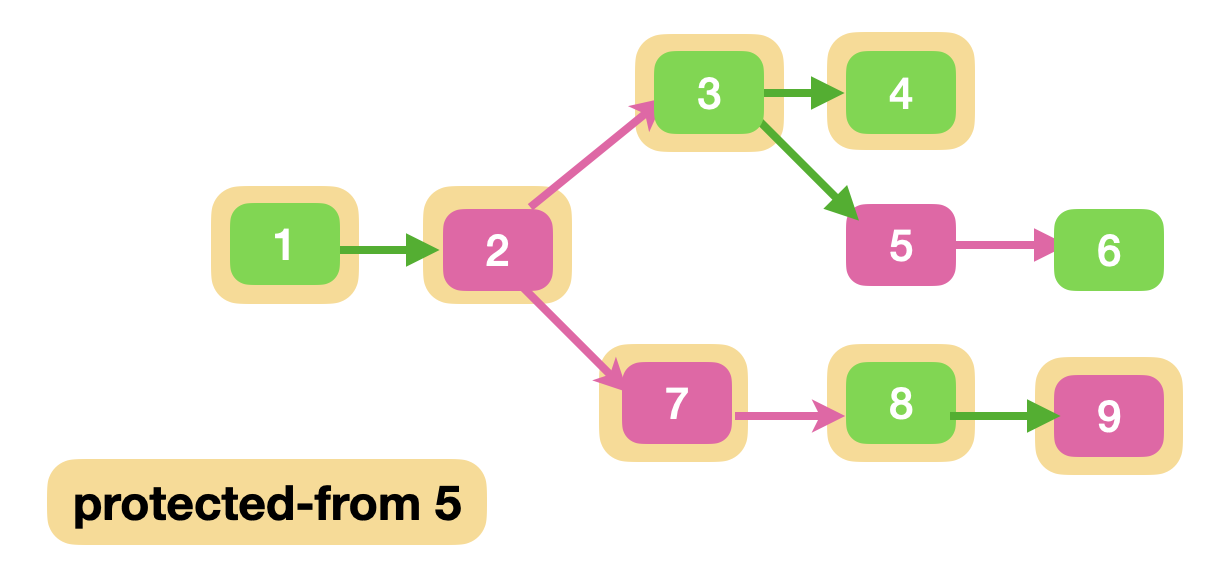
\includegraphics[width=\linewidth]{diagrams/prfA.png}
} 
&
\resizebox{4.5cm}{!}{
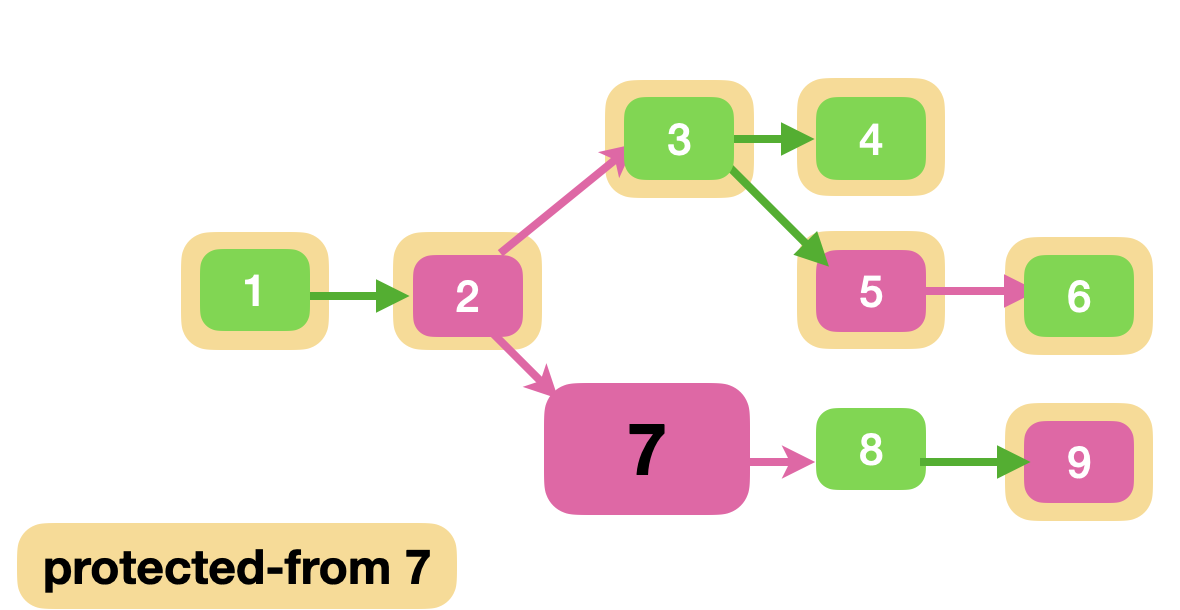
\includegraphics[width=\linewidth]{diagrams/prfB.png}
} 
&
\resizebox{4.5cm}{!}{
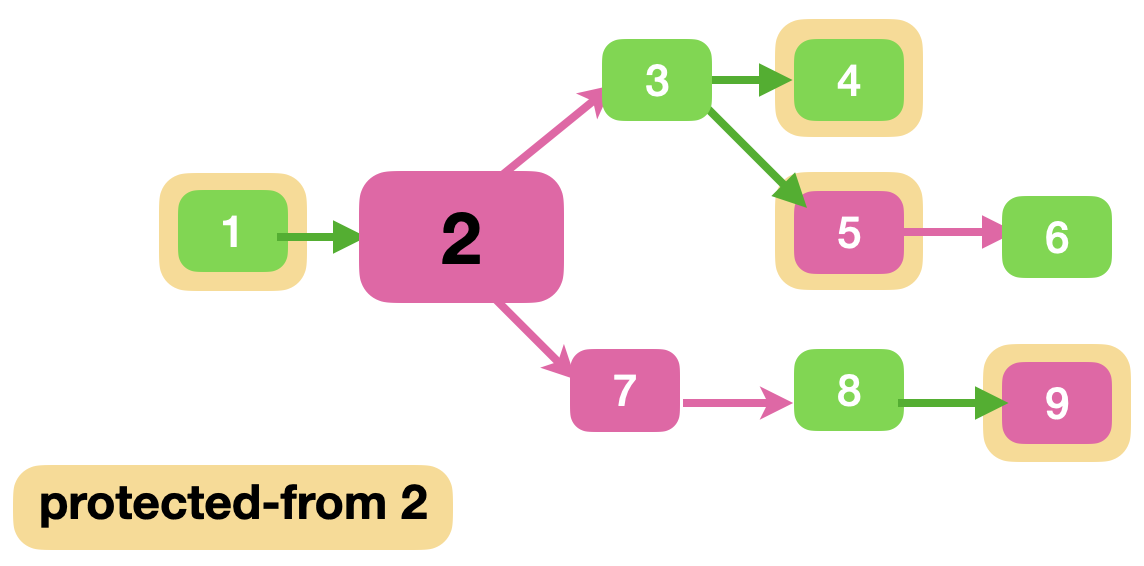
\includegraphics[width=\linewidth]{diagrams/prfC.png}
} 
\\
\hline
protected from $o_5$
&
protected from $o_7$
&
protected from $o_2$
\\
\hline \hline
\end{tabular}
   \caption{Relative Protection. Pink objects are external, and green objects are internal.}
   \label{fig:ProtectedFrom}
 \end{figure}
 
 

%Note that $o_8$ is not protected from $o_2$ because there is a path from $o_2$ to $0_8$ which only traverses external objects. Note also, that even though $o_9$ is external, it is protected from $o_7$.
Note that $o_6$ is not protected from $o_2$. 
Namely, even through there are some internal objects on the path from $o_2$ to $o_6$, in our current model, these objects are not sufficient to prevent eventual, unmitigated access of $o_2$ to $o_6$: it is possible for $o_2$ to make a call to $o_3$, and then this call to return $o_5$. Once $o_2$ has access to $o_5$, it can also get access to $o_6$. 

\vspace{.1in}

We now introduce the concept of (absolute) protection.
An object is protected, if it is protected from all locally reachable {external} objects. This can also be understood as 
``protected from the top frame''. \footnoteSD{TODO: motivate; many external objects, no matter which one has unprotected access to an object }
 
\begin{definition}[Satisfaction 
of Assertions -- Protected] 
\label{def:chainmail-protection}
\label{sect:semantics:assert:prt}
-- continuing definitions from \ref{def:chainmail-semantics} and \ref{def:chainmail-protection-from}:
\begin{enumerate}
\item
$\satisfiesA{M}{\sigma} {\inside {\re}}$  \ \ \ iff \ \ \ 
\begin{enumerate}
\item
{$\forall \alpha.[ \  \LRelevant {\alpha}  {\sigma}\ \wedge\ { \satisfiesA{M}{\sigma}{\external \alpha}} \ \ \Longrightarrow \ \  \satisfiesA{M}{\sigma}{\protectedFrom{\re} {{\alpha}}}\ ] $}, \ \ \ and 
\item
$\satisfiesA{M}{\sigma}{\extThis}\ \ \Longrightarrow\ \ \forall x\!\in\! \sigma.\ \satisfiesA{M}{\sigma}{x\neq \re}$
\end{enumerate}
\end{enumerate}
\end{definition} 
 
% TODO explain
  Figure \ref{fig:Protected} illustrates %the concept of 
  protection. The heap in all three panes is the same as in  Fig \ref{fig:LReachable} and 
 Fig \ref{fig:ProtectedFrom}. The left pane's  top frame is $\phi_1$; it has  one variable, \prg{this}, pointing to $o_1$.  The middle pane's  top frame is $\phi_2$; it has two  variables,   \prg{this} and \prg{x} pointing to $o_3$ and  $o_7$ resp. The right pane's  top frame is $\phi_3$; it has two  variables,  \prg{this} and \prg{x}, pointing to $o_7$ and $o_3$, resp.  

\begin{figure}[htb]
\begin{tabular}{|c|c|c|}
\hline \\
\resizebox{4.5cm}{!}{
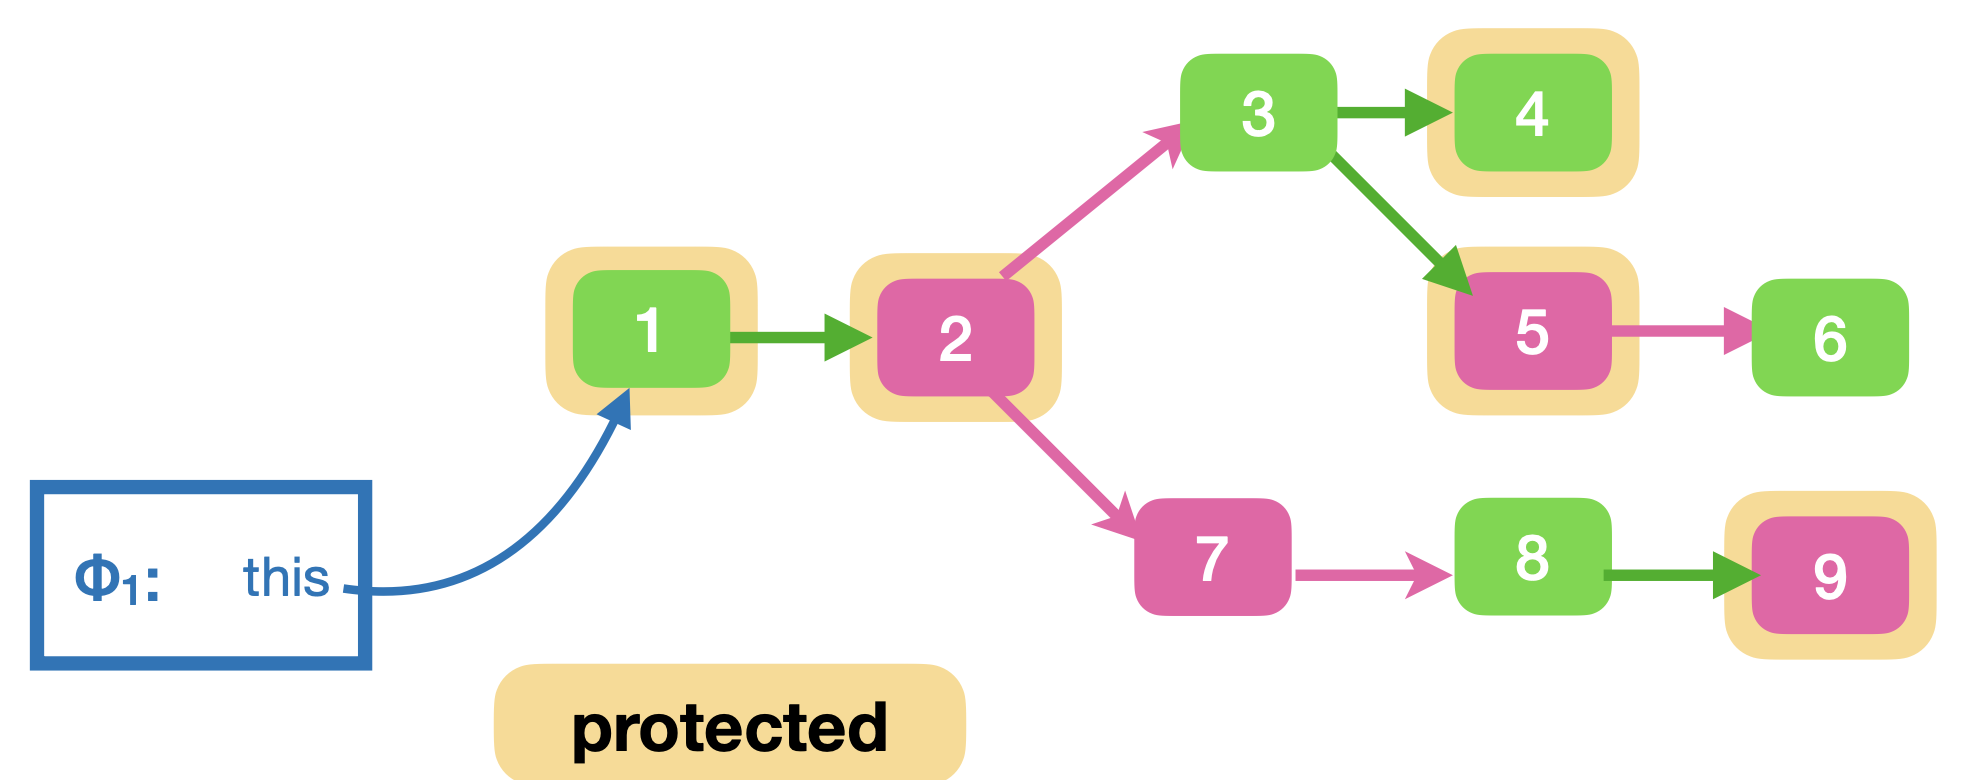
\includegraphics[width=\linewidth]{diagrams/prtFirst.png}
} 
&
\resizebox{4.5cm}{!}{
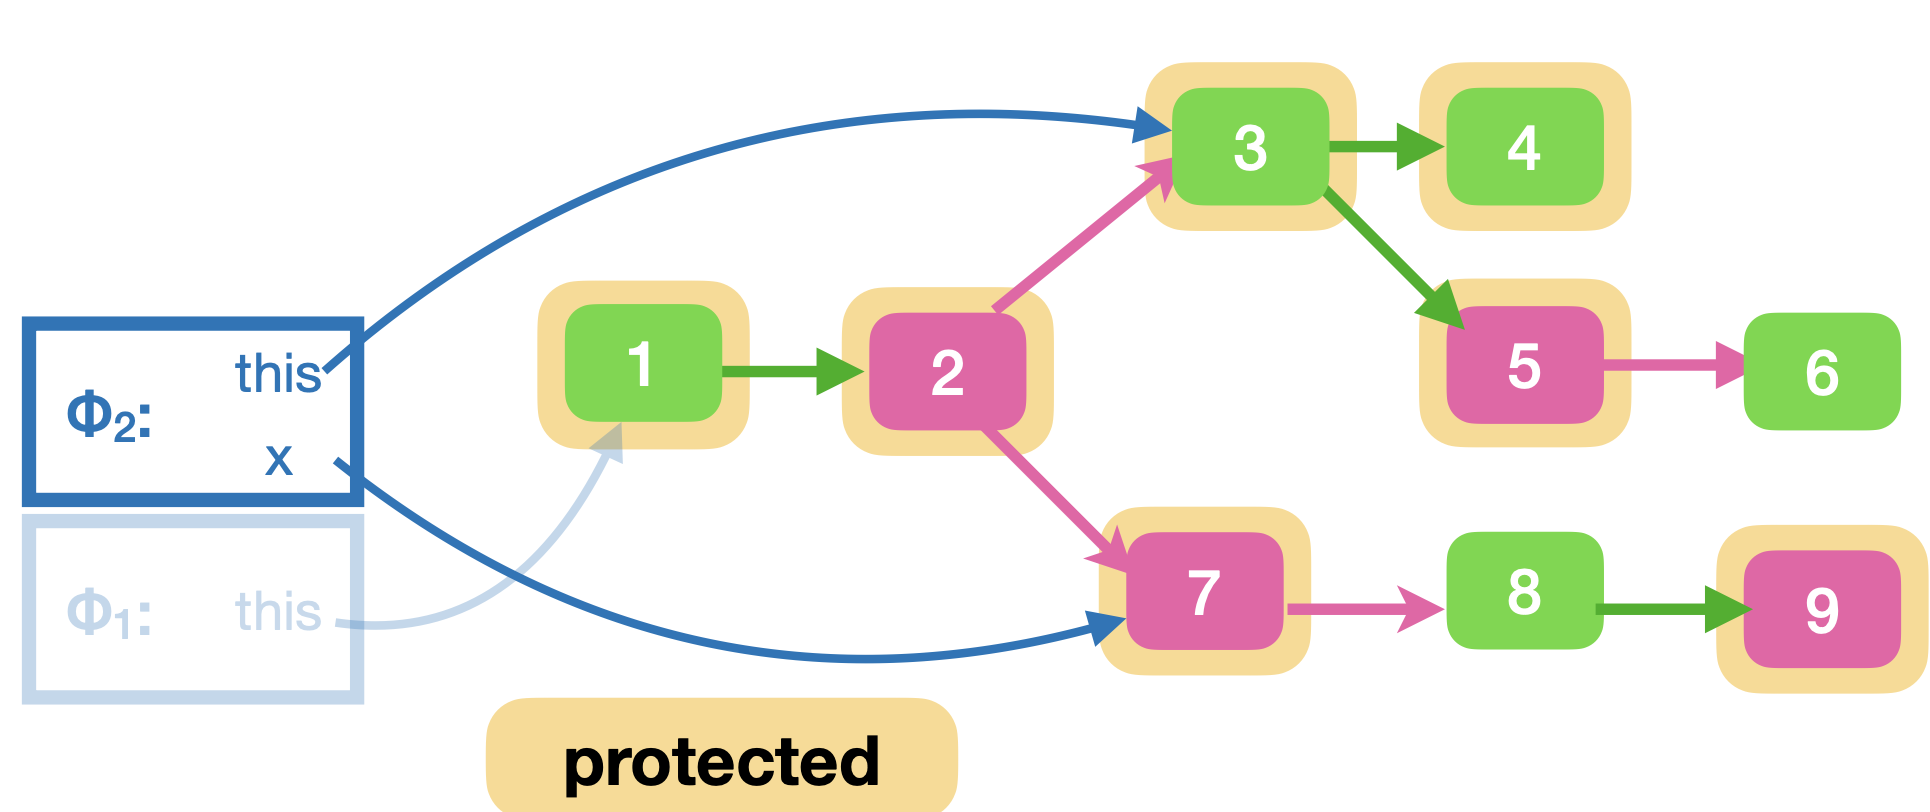
\includegraphics[width=\linewidth]{diagrams/prtSecond.png}
} 
&
\resizebox{4.5cm}{!}{
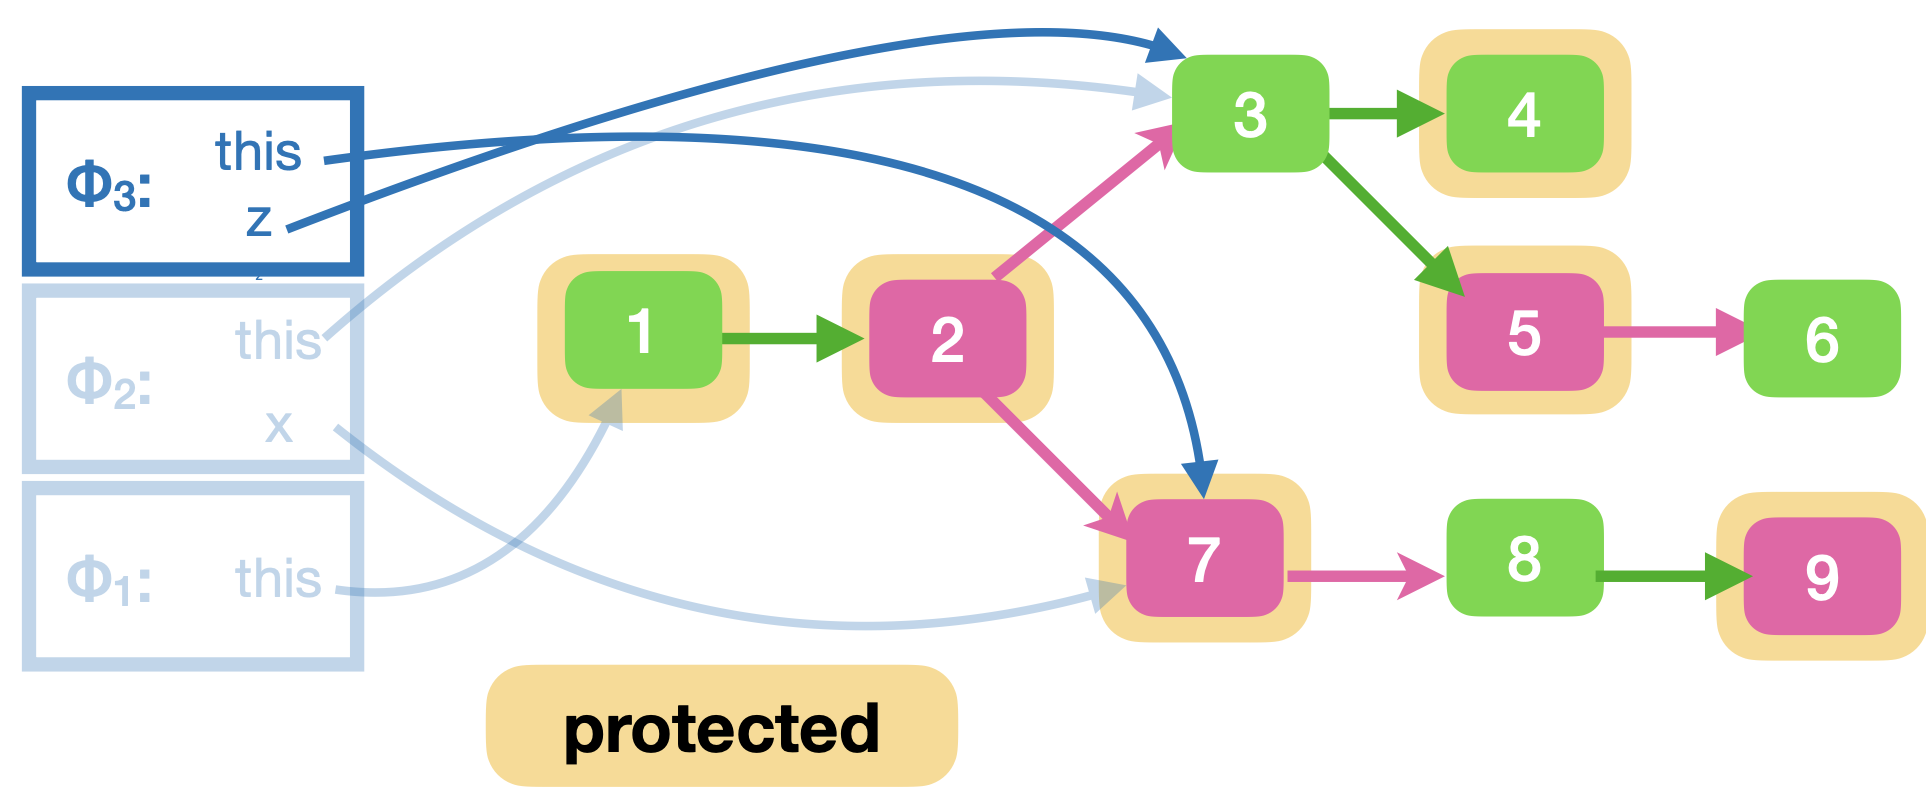
\includegraphics[width=\linewidth]{diagrams/prtLast.png}
} 
\\
\hline
protected  with top frame $\phi_1$ &
protected  with top frame $\phi_2$
&
protected  with top frame $\phi_3$
\\
\hline \hline

\end{tabular}
   \caption{Protected \\
 }
   \label{fig:Protected}
 \end{figure}
 
 
The locally reachable objects from $\phi_1$ were highlighted in the middle pane of Fig \ref{fig:LReachable}, while the locally reachable object from $\phi_2$ as well as from $\phi_3$ were  highlighted in the right pane of that Figure. 
We highlight the protected objects in each pane with a golden halo.
 Note that $o_3$ is protected from $\phi_2$, but is not protected from $\phi_3$. This is so, because \prg{this} in $\phi_3$ is external, and  $o_3$ is an argument to the call. That means, that during the call, $o_7$ may obtain unmitigated access (permission?) to $o_3$. 
 
 \subsection{Preservation of Satisfaction across Method Calls and Returns}

\sdN{Satisfaction of an assertion depends on the contents of the heap, and the map of local variables to addresses in the top frame of that stack. 
It is useful to know under what conditions  satisfaction of  assertions is preserved across changes to the state.
In particular, what if the heap remains the same, and the assertion has no free variables?
Usually, in such cases satisfaction is preserved across pushing/popping of frames on the stack.
However, in our assertion language, assertions may talk about protection, and as we have already seen in Fig. 4, this property is affected when we push of pop frames.

In this section we will study the preservation of satisfaction across pushing and popping of frames.

Lemma \ref{l:assrt:unaffect}  says that satisfaction of an assertion is not affected by replacing a variable by its value, nor by changing the continuation in a state.


\begin{lemma}
\label{lemma:addr:expr}
\label{l:assrt:unaffect}
For all $M$, $\sigma$, $\alpha$, $x$, $\re$, $A$:

\begin{enumerate}
\item
\label{one:ad:exp}
$ \satisfiesA{M}{\sigma[x\mapsto \alpha]}{A}   \ \ \ \Longleftrightarrow\ \ \ \satisfiesA{M}{\sigma}{A[\alpha/x]} $ 
\item
$\eval{M}{\sigma}{{\re}}{\alpha}  \ \ \ \Longrightarrow\ \ \  [ \ \satisfiesA{M}{\sigma}{A} \  \Longleftrightarrow\   \  \satisfiesA{M}{\sigma}{A[\alpha/\re]} \  \  ]$
\item
$ \satisfiesA{M}{\sigma}{A}   \ \ \ \Longleftrightarrow\ \ \ \satisfiesA{M}{\sigma[\prg{cont}\mapsto stmt]}{A}$ 
\end{enumerate}

\end{lemma}

A corollary of   lemma \ref{l:assrt:unaffect}.\ref{one:ad:exp} is that $\satisfiesA{M}{\sigma}{A}  \ \ \Longleftrightarrow  \ \   \satisfiesA{M}{\sigma}{A[{\interpret \sigma x}/x]}$.


\subsubsection{Stable, and Positive Assertions}\footnote{BETTER NAME?}  Stable assertions are those which   do not contain the requirement $\inside{\_}$ are called {\emph {stable}}. 
Their satisfaction is preserved against pushing and popping of frames.
Positive Assertions are those where protection appears only in positive positions.
Their satisfaction is preserved against pushing of frames.

%%%\newcommand{\lclSPACE}{\ \ \ \ \ }   %%%KJX: ALREADY DEFINED IN definitions.sty

% An assertion is {\emph {stable}}, written as $\Stable A$ if it does not contain $\inside {\re}$ assertions:
\begin{definition}
\label{def:Basic}
%\begin{figure}[hbt]
[$\Stable{\_}$] assertions: %  defined below

$
\begin{array}{l}
 \begin{array}{lll}
  \Stable {\inside{\re}}  \triangleq  false & \lclSPACE &   \Stable {\protectedFrom \re {\overline {u}}} =  
  \Stable  {\internal \re} =  %   \PushAS y  {(\external \re)} & \triangleq &   {\external \re}
    \Stable {\re}=   
     \Stable {\re:C}\   \triangleq \    true
 \end{array}
  \\
 \begin{array}{lcl}
 \Stable  {A_1  \wedge  A_2}\  \triangleq\     \Stable  { A_1}  \wedge    \Stable  {A_2}    &
\lclSPACE  &  
 \Stable  {\forall x:C.A} =\Stable  {\neg A} \   \triangleq\   \Stable A
 \end{array}
 \end{array}
$
\label{f:Basic}
\end{definition}

 
% An assertion is {\emph {stable}}, written as $\Stable A$ if it does not contain $\inside {\re}$ assertions:
\begin{definition}
\label{def:Pos}
%\begin{figure}[hbt]
[$\Pos{\_}$] assertions: %  defined below

$
\begin{array}{l}
 \begin{array}{l}
  \Pos {\inside{\re}} =  \Pos {\protectedFrom \re {\overline {u}}} =  
  \Pos  {\internal \re} =   
    \Pos {\re}=   
     \Pos {\re:C}\   \triangleq \    true
 \end{array}
  \\
 \begin{array}{lll}
 \Pos  {A_1  \wedge  A_2}\  \triangleq\     \Pos  { A_1}  \wedge    \Pos  {A_2}   \  &
      
 \Pos  {\forall x:C.A}   \triangleq\   \Pos A
\   &
  \Pos {\neg A}  \triangleq \Neg A
 \end{array}
 \\
 \\
  \begin{array}{ll}
  \Neg {\inside{\re}}\  \triangleq \    false &    \Neg {\protectedFrom \re {\overline {u}}} =  
  \Neg  {\internal \re} =   
    \Neg {\re}=   
     \Neg {\re:C}\   \triangleq \    true
 \end{array}
  \\
 \begin{array}{lll}
 \Neg  {A_1  \wedge  A_2}\  \triangleq\     \Neg  { A_1}  \wedge    \Neg  {A_2}   \ \   
 &    
 \Neg  {\forall x:C.A}   \triangleq\   \Neg A \ \ 
&
  \Neg {\neg A}  \triangleq \Pos A
 \end{array}

 \end{array}
$
\label{f:Pos}
\end{definition}

As we see in the following lemma, stability is stronger than positive and also negative protection. On the other hand, positive protection does not imply stability, consider, \eg the assertion $\inside \re$.

\begin{lemma}
For all   assertions $A$  
\label{l:preserve:asrt}
 
\begin{itemize}
\item 
$\Stable{A}\ \ \ \  \Longrightarrow \ \  \ \  \Pos{A}\  \wedge\  \Neg{A} $
\end{itemize}
\end{lemma}

Lemma \ref{l:preserve:asrt}  is about preservation of satisfaction of   assertions  across pushing and popping of frames:

\begin{lemma}
For all  states $\sigma$ and frames $\phi$, and for all assertions $A$ such that $ fv(A)=\emptyset$:
\label{l:preserve:asrt}
 
\begin{itemize}
\item 
$\Stable{A}\ \ \ \  \Longrightarrow \ \  \ \  [\ \ M, \sigma \models A \ \ \Longleftrightarrow \ \  M,{\PushSLong \phi \sigma} \models A\ \ ]$
\item 
$\Pos{A}\ \ \ \  \Longrightarrow \ \  \ \  [\ \ M, \sigma \models A \ \ \Longrightarrow \ \  M,{\PushSLong \phi \sigma} \models A\ \ ]$
\item 
$\Neg{A}\ \ \   \Longrightarrow \ \  \ \  [\ \ M, \sigma \models A \ \Longleftarrow \ \  M,{\PushSLong \phi \sigma} \models A\ \ ]$

\end{itemize}
\end{lemma}
 }
  
   
 \subsubsection{Viewpoints and Protection}
 
 
{The examples in Fig. \ref{fig:Protected} demonstrate that % validity of assertions which refer to 
 protection may be affected by the pushing and popping of frames on the stack. For example, $o_3$ was not protected with top frame $\phi_1$,   became protected when we pushed the frame $\phi_2$,  and again, is no longer protected when we push $\phi_3$ on the stack. 
 
Below we define 
$\pushSymbolAA$, which  translates an assertion from the viewpoint of the callee, to that of the caller:
it applies to assertions and sequences of variables:  $\PushAS y A$   guarantees that $A$ will hold when the values of $y$ have been pushed onto a new frame:
 thus, $\PushAS y A$ is \emph{hypothetical}.
 % : if a state satisfies $\PushAS y A$, then after pushing
% onto that state a frame which contains the values  of $\overline y$, assertion $A$ will hold. }
% $\pushSymbolAA$ is the counterpart to $\pushSymbol$, which we had defined for states, \cf Lemma \ref{lemma:push:ass:state}

% Lemma \ref{lemma:vars:to:addresses} says that: (1)Validity of an assertion $A$ in the context of a state $\sigma$ implies  validity of the assertion resulting  from substituting free variables according to the top frame ($A[\sigma]$)}.
%%(2) A bounded execution step (thus not returning from current call)
%in an external state preserves absolute protection.
%(3) An objects which is protected from  the receiver and arguments of a method call, is protected   after the corresponding frame has been pushed onto the stack.

The  $\pushSymbolAA$  operator is  defined in Fig. \ref{f:Push}. Only the first equation is interesting, i.e.  $\PushAS y {(\inside x)}$: For 
$x$ to be protected from the viewpoint of the callee, it should be protected from all the call's arguments,
\ie  $\protectedFrom x {\overline {y}}$. 
In all other cases,   $\pushSymbolA$  leaves simple $\re$'s unmodified %(i.e. the second to sixth equation), 
 or is applied to the sub-assertions. % (i.e. the seventh to eleventh equation).

\begin{definition}
\label{def:push}
%\begin{figure}[hbt]
[The $\pushSymbolAA$  operator] is  defined below

$
\begin{array}{c}
\begin{array}{l}
\begin{array}{rclcrcl}
  \PushAS y {(\inside \re)} & \triangleq &  \protectedFrom \re {\overline {y} }
  & \ \ \  \ &
  \PushAS y   {(A_1  \wedge  A_2)} & \triangleq &  (\PushAS y  { A_1})  \wedge  ( \PushAS y  {A_2} )  
\\ 
 \PushAS y {(\protectedFrom \re {\overline {u}})} &  \triangleq& \protectedFrom \re {\overline {u}} 
  & &
 \PushAS y  {(\forall x:C.A)} & \triangleq & \forall x:C.({\PushAS y A} )  
  \\  
  \PushAS y  {(\external \re)} &  \triangleq & {\external \re}  %   \PushAS y  {(\external \re)} & \triangleq &   {\external \re}
  & & 
  \PushAS y  {(\neg A)} &  \triangleq & \neg( {\PushAS y A} )  
    \\
     \PushAS y  {\re} &  \triangleq&   \re %    \PushAS y  {(\internal \re)} &  \triangleq & {\internal \re}
    & &
    \PushAS y  {(\re:C)} &  \triangleq&   \re:C 
 \end{array}
\end{array}
\end{array}
$
% \caption{The $\pushSymbolAA$  operator  } 
\label{f:Push}
%\end{figure}
\end{definition}

 


\newcommand{\sigmas}{\widetilde \sigma}



\vspace{.1cm}

 Lemma \ref{lemma:push:ass:state}  states that $\pushSymbolAA$ is the counterpart to the states' operator $\pushSymbol$:
 %states the guarantees given by $\pushSymbolAA$: \  
 (1) If \ %the current state 
$\sigma$ satisfies  $\PushAS y A$, then   { the callee state (after pushing a frame with the values of $\overline y$) 
will satisfy $A$}. %after pushing a frame with the values of $\overline y$ (here $\PushS {y} {\sigma}$)
(2) is the opposite: {If the callee state (in which we pushed a frame with the values for $\overline y, \overline z$) satisfies $A$, then the
caller state will satisfy 
% (here , conversely,   if a state satisfies  $A$ after a top frame containing the  values of $\overline y$  and some other variables has been pushed % (here \PushSLong {(\overline y, \overline z)} \sigma), 
$\PushAS {y} {A}$. } % will hold {in the caller state}. % after popping that frame.
%, and mapping the free variables of $A$ to their values  in the state  before.


\begin{lemma} 
\label{lemma:push:ass:state}
For any state  $\sigma$, assertion $A$, and variables   $\overline y, \overline z$, disjoint with one another:
\\
If  $\fv(A)=\emptyset$, then
\begin{enumerate}
 \item
 \label{lemma:push:ass:state:one}
$M, \sigma \models \PushAS {y} {A}\ \ \ \ \ \ \  \ \ \    \Longrightarrow  \ \ \ \ M,  \PushS {y} {\sigma}   \models A$
\item
\label{lemma:push:ass:state:two}
$M, { \PushSLong {(\overline y, \overline z)} {\sigma} } \models\  A \  \ \ \ \Longrightarrow  \ \ \ \ M,  \sigma \models  \PushAS  {y} {A}$
\end{enumerate}
\end{lemma}
 \footnoteSD{OLD form:
 \\
 \begin{enumerate}
 \item
 \label{lemma:push:ass:state:one}
$M, \sigma[\overline{x \mapsto \alpha} ] \models \PushAS {y} {A}\ \ \ \     \Longrightarrow  \ \ \ \ M,  \PushS {y} {(\sigma[\overline{x \mapsto \alpha}])}   \models A$
\item
\label{lemma:push:ass:state:two}
$M, {(\PushSLong {(\overline y, \overline z)} {(\sigma[\overline{x \mapsto \alpha} ] )})}  \models\  A \  \ \ \ \Longrightarrow  \ \ \ \ M,  \sigma[\overline{x \mapsto \alpha} ] \models  \PushAS  {y} {A}$
\end{enumerate}
}


\noindent
\textbf{NOTES} \notesep 
{We require   $\fv(A)=\emptyset$ in order to be accommodate for the difference between variable maps in $\sigma$ and  $\PushS {y} {\sigma}$.}
%We could, instead,  require that $fv(A)=\overline x$, \ $\overline x \notin \sigma$, \ $\overline x \notin  \PushAS {y} {A}$, and   assert that (1)\ $M, \sigma[\overline{x \mapsto \alpha} ] \models \PushAS {y} {A}\  \Longrightarrow   \ M,  \PushS {y} {(\sigma[\overline{x \mapsto \alpha}])}   \models A$, and similarly for (2).}
%In both (1) and (2), we  use the renaming $\sigma[\overline{x \mapsto \alpha} ]$ to ensure that the free variables of $A$ are mapped to the same values in the caller's and the callee's frame.
 \notesep 
To simplify notation,  we lifted % the $\models$ 
judgements to sets of states: If  $\sigmas$ is a set of states,  then
$M,   \sigmas \models A$ stands for  $\forall\sigma\! \in\! \sigmas.[\, M,\sigma \models A \, ]$.    

\footnoteSD{\vspace{.1cm}
\noindent 
\blue{\textbf{Comment} The $ \pushSymbol$ operator reminds me of the magic wand. Namely, $-\!-\!*$ is spatial and heap based:  the assertion $A -\!-\!* A'$ says: if you combine with a heap that satisfies $A$, then the complete heap will satisfy $A'$. While $\PushASLong {\_} {\_}$ is temporal and  stack based: the assertion  $\PushAS {y} A$ says that if you push a frame with range the values of $\overline y$, then $A$ will hold. \textbf{End Comment} }
}
%{{I am surprised that $ \pushSymbol$  only affects  ${\inside x}$, and leaves all else unmodified,}}

 

 
